\documentclass[3p,twocolumn]{elsarticle}

\usepackage{graphicx}
\usepackage{color}
\usepackage{url}
\usepackage{float}
\usepackage{listings}
\usepackage[small,it]{caption}
\usepackage{ifpdf}
\usepackage{pdfsync}
\usepackage{hyperref}
\usepackage{xspace}

\setlength\parskip{-0.015em}
\setlength\parsep{-0.15em}

\newenvironment{shortlist}{
	\vspace*{-0.85em}
  \begin{itemize}
 \setlength{\itemsep}{-0.3em}
}{
  \end{itemize}
	\vspace*{-0.6em}
}

\begin{document}

\title{Understanding Application-Level Interoperability: Scaling-Out
  MapReduce Over High-Performance Grids and Clouds}

% author order is inverse alphabetical, because we have April... ;-)
% is that a good joke? people at the end of the list might complain =:->
     \author{Saurabh Sehgal$^1$, Miklos Erdelyi$^{3,4}$, Andre Merzky$^{1}$, Shantenu Jha$^{*1,2}$
       \\
       \small{\emph{$^{1}$Center for Computation \& Technology, Louisiana State University, USA}}\\
       \small{\emph{$^{2}$Department of Computer Science, Louisiana State University, USA}}\\
       \small{\emph{$^{3}$Department of Computer Science \& Systems
           Technology, University of
           Pannonia, Veszprem, Hungary}}\\
       \small{\emph{$^{4}$Computer \& Automation Research Institute of
           the Hungarian Academy of
           Sciences}}\\
       \small{\emph{$^{*}$Contact Author \texttt{sjha@cct.lsu.edu}}}
       \upp\upp\upp\upp\upp
       }

\newif\ifdraft
%\drafttrue
\ifdraft
 \newcommand{\amnote}[1]{     {\textcolor{magenta} { ***AM: #1 }}}
 \newcommand{\jhanote}[1]{    {\textcolor{red}     { ***SJ: #1 }}}
 \newcommand{\miklosnote}[1]{ {\textcolor{blue}    { ***ME: #1 }}}
 \newcommand{\ssnote}[1]{     {\textcolor{blue}    { ***SS: #1 }}}
\else
 \newcommand{\amnote}[1]{}
 \newcommand{\jhanote}[1]{}
 \newcommand{\miklosnote}[1]{}
 \newcommand{\ssnote}[1]{}
\fi

\newcommand{\sagamapreduce}{SAGA-MapReduce\xspace}
\newcommand{\smr}{\sagamapreduce}
\newcommand{\mr}{MapReduce\xspace}
\newcommand{\tc}{$T_c$\xspace}
\newcommand{\wc}{wordcount\xspace}
\newcommand{\Wc}{Wordcount\xspace}

\newcommand{\dn}{\vspace*{0.33em}}
\newcommand{\dnn}{\vspace*{0.66em}}
\newcommand{\dnnn}{\vspace*{1em}}
\newcommand{\uppp}{\vspace*{-1em}}
\newcommand{\upp}{\vspace*{-0.66em}}
\newcommand{\up}{\vspace*{-0.33em}}
\newcommand{\shift}{\hspace*{1.00em}}

\newcommand{\T}[1]{\texttt{#1}}
\newcommand{\I}[1]{\textit{#1}}
\newcommand{\B}[1]{\textbf{#1}}
\newcommand{\F}[1]{\B{[FIXME: #1]}}
\newcommand{\TODO}[1]{\textcolor{red}{\B{TODO: #1}}}

\newcommand{\ssh}[1]{\T{ssh}\xspace}
\newcommand{\scp}[1]{\T{scp}\xspace}
\newcommand{\sshfs}[1]{\T{sshfs}\xspace}


%\maketitle
\begin{abstract}
  Application-level interoperability is defined as the ability of an
  application to utilize multiple distributed heterogenous resources.
  Such interoperabilty is becoming increasingly important with
  increasing volumes of data, multiple sources of data as well as
  resource types.  The primary aim of this paper is to understand
  different ways in which application-level interoperability can be
  provided across distributed infrastructure. We achieve this by (i)
  Using the canonical \wc application, using 
  SAGA-based \mr that scales-out across clusters, clouds and HPC resources, (ii)
  establishing % how SAGA enables the 
  the execution of \wc application using
  \mr and other programming models such as Sphere concurrently.  We
  also discuss how a SAGA-based \mr enables a version of \mr which in
  addition to being interoperable across different distributed
  infrastructures, also provides user-level control of the relative
  placement of compute and data.  We provide performance
  measures and analysis of \sagamapreduce when using multiple,
  different, heterogeneous infrastructures concurrently for the same
  problem instance.

% However, we do not strive to provide a rigorous performance
% model, but to provide a proof-of-concept of application-level
% interoperability and illustrate its importance.

\end{abstract}
\maketitle


\section{Introduction}
\label{sec:intro}

% Although clouds are a nascent infrastructure, there is a ground swell
% in interest to adapt these emerging powerful infrastructure for
% large-scale scientific applications~\cite{montagecloud}. Inevitably,
% and as with any emerging technology, the unified concept of a cloud --
% if ever there was one, is evolving into different flavors and
% implementations, with distinct underlying system interfaces, semantics
% and infrastructure. For example, the operating environment of Amazon's
% cloud (EC2) is very different from that of Google's
% cloud. Specifically for the latter, there already exist multiple
% implementations of Google's BigTable, such as HyberTable, Cassandra
% and HBase. There is bound to be a continued proliferation of such
% cloud based infrastructure; this is reminiscent of the plethora of
% grid middleware distributions.

There are numerous scientific applications that either currently
utilize, or need to utilize data and resources distributed over vast
heterogeneous infrastructures and networks with varying speeds and
characteristics.  Many scientific applications are, however, designed
with a specific infrastructure; such dependence and
tight-coupling to specific resource types and technologies is, in a
heterogeneous distributed environment, not an optimal design choice.
In order to leverage the flexibility of distributed systems and to
gain maximum runtime performance, applications must shed their
dependence on single infrastructure for all of their computational and
data processing needs. For example, the Sector/Sphere data cloud is
exclusively designed to support data-intensive computing on high speed
networks, while others, like the distributed file systems GFS/HDFS,
assume limited bandwidth among infrastructure nodes ~\cite{GFS, HDFS}.
Thus, for applications to efficiently utilize heterogeneous
environments, abstractions must be developed for the efficient
utilization of and orchestration across such distinct distributed
infrastructure.

% We define the ability of an application to utilise multiple
% distributed heterogenous resources as application-level interop
% \jhanote{Introduce IDEAS and explain how ``I'' is the basis upon
%   which DEAS are built/predicated}

In addition to issues of performance and scale addressed in the
previous paragraph, the transition of existing distributed programming
models and applications to emerging and novel distributed
infrastructure must be as seamless and as non-disruptive as
possible.  A fundamental question at the heart of all these
considerations is the question of how scientific applications can be
developed so as to utilize as broad a range of distributed systems as
possible, without vendor lock-in, yet with the flexibility and
performance that scientific applications demand.

% Additionally, there are infrastructure specific features --
% technical and policy, that might influence the design of PM and
% PS. For example, EC2 -- the archetypical cloud system, has a
% well-defined cost model for data transfer across {\it its}
% network. Hence, any PM for clouds should be cognizant of the
% requirement to programmatically control the placement of compute and
% data relative to each other -- both statically (pre-run time) and
% dynamically (at run-time).  In general, for most cloud applications
% the same computational task can be priced very differently for
% possibly the same performance; conversely, the same computational
% task can have very different performance for the same price.

We define Application Level Interoperability (\I{ALI}) as a feature
that arises, when other than say compiling, there are no further
changes required of the application to utilize a new platform.
% If service-level interoperability can be considered as weak
% interoperability, ALI can be considered to be {\it strong}
% interoperability.\amnote{weak versus strong is badly motivated
% here - add reference?}
The complexity of providing ALI varies and depends upon the
application under consideration.  For example, it is somewhat easier
for simple ``distribution unaware'' applications to utilize multiple
heterogeneous distributed environments, than for applications where
multiple distinct and possibly distributed components need to
coordinate and communicate.

% A pre-requisite for ALI is infrastructure independent programming.

\paragraph{The Case for Application-level Interoperability}

In either case, ALI is not only of theoretical interest. There exist
many applications which involve large volumes of data on distributed
heteregenous resources and which benefit from ALI. For examples, the
Earth-Science Grid involves peta to exa-bytes of data, and one thus
cannot move all data (given current transfer capabilities), nor
compute at a centralized location.  Thus there is an imperative to
operate on the data {\it in situ}, which in turn involves computation
across heteregenous distributed platforms as part of the same
application.

In addition, there exist a wide range of applications that have
decomposable but heterogeneous computational tasks. It is conceivable,
that some of these tasks are better suited for traditional grids,
whilst some are better placed in cloud environments.  The LEAD
application, as part of the VGrADS project provides a prominent
example\footnote{\url{http://vgrads.rice.edu/presentations/VGrADS_overview_SC08pdf.pdf}}.
Due to different data-compute affinity requirement amongst the tasks,
some workloads might be better placed on a cloud~\cite{jha_ccpe09},
whilst some may optimally be located on regular grids. Complex
dependencies and inter-relationships between sub-tasks make this often
difficult to determine before run-time.

Last, but not least, in the rapidly evolving world of clouds, there is
as of yet little business motivation for cloud providers to define,
implement and support new/standard interfaces. Consequently, there is
a case to be made that by providing ALI, such barriers can be overcome
and cross-cloud applications can be easily achieved.

Currently, many programming models and abstractions are tied to a
specific back-end infrastructure.  For example, Google's MapReduce,
which is tied to Google's file system, or Sphere\cite{sectorsphere09}
which is linked to the Sector file system.  It is often the case that
an application maybe significantly better suited to a specific
programming model; similarly a specific programming model maybe
optimised for a specific infrastructure. However, where this is not
necessarily the case, or more importantly, when different
applications or programming models can utilise ``non-native''
infrastructure, the ability to mix-and-match across the layers of
applications, programming models and infrastructure should be
supported.  Ideally, an application should be able to utilize any
programming model, and any programming model should be executable on
any underlying infrastructure.  Thus there is a need to investigate
interoperability of different programming models for the same
application on different systems.

We will
work with MapReduce and an application based on \mr -- the canonical
\wc application.  We use SAGA --- “Simple API for Grid Applications''
(see Sec.~\ref{sec:saga}) as the programing system for distributed
applications.  In Ref.~\cite{saga_ccgrid09}, we
implemented a \mr based \wc application using SAGA.  We
demonstrated that the SAGA-based implementation is infrastructure
independent, whilst still providing control over deployment,
distribution, run-time decomposition and data/compute co-location.  We
demonstrated that \sagamapreduce is interoperable on traditional
(grids) and emerging (clouds) distributed infrastructure
\I{concurrently and cooperatively towards a solution of the same
  problem instance}.
% Our approach was to % take \sagamapreduce and to
% use the \I{same} %instance of \sagamapreduce to solve the same
% instance of the {\wc}ing problem, by using different worker
% distributions over clouds and grid systems.

The primary focus of this paper is to understand, demonstrate and
investigate different types of ALI. We build upon and use SAGA-based
MapReduce as an exemplar to discuss multiple levels and types of
interoperability that can exist between infrastructures. We use
\sagamapreduce and SAGA-based Sphere on different infrastructure. We
will also show that our approach to ALI helps break the coupling
between progamming models and infrastructure on the one hand, whilst
providing empirically-driven insight about the performance of an
application with different programming models.

% and thereby also test for interoperability between different flavors
% of clouds as well as between clouds and grids.

% this involved the concurrent execution of simple,
% embarrassingly-parallel data-analysis tasks.

This paper is structured as follows: Section~\ref{sec:saga} gives a
short overview over those SAGA extensions which enable specifically
the ALI work discussed in this paper.  Section~\ref{sec:mr} describes
our \smr implementation.  Section~\ref{sec:interop} discusses the
different levels of ALI we investigate and demonstrate, with more
details on the experiments provided in Section~\ref{sec:exp}.
Section~\ref{sec:discuss} concludes the paper with a discussion of the
results.

% Thanks to the ease of
% developing SAGA “Adaptors”, developers can provide SAGA the interfaces
% to interact with widely different infrastructures simultaneously
% throughout the execution of a single application.

% It is worth mentioning that most
% data-intensive scientific applications fall into this category e.g.,
% high-energy and LIGO data-analysis.


\section{SAGA}
\label{sec:saga}

The SAGA~\cite{saga-core, Kaiser:2006qp} programming system provides a
high level API that forms a simple, standard and uniform interface for
the most commonly required distributed functionality.  SAGA can be
used to program distributed applications~\cite{saga_escience07,
saga_tg08} or tool-kits to manage distributed
applications~\cite{Luckow:2008xy}, as well as implement abstractions
that support commonly occurring programming, access and usage
patterns.

\begin{figure}[t]
 \dnnn
 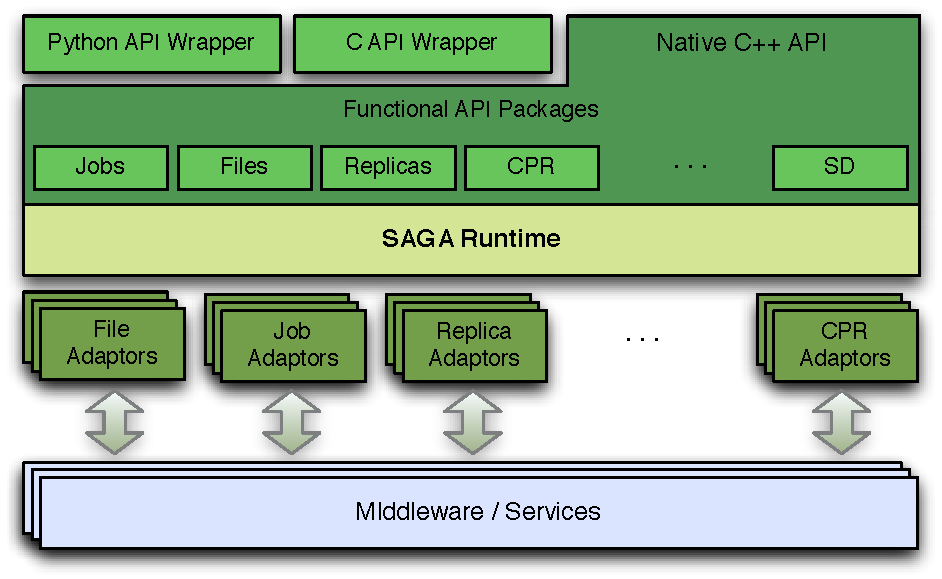
\includegraphics[scale=0.5]{figures/saga-figure02.pdf}
 \caption{The SAGA runtime engine dynamically dispatches high level
          API calls to a variety of middlewares.}
 \label{fig:saga}
\end{figure}

Fig.~\ref{fig:saga} provides an overview of the SAGA programming
system's architecture.  The SAGA API covers job submission, file
access and transfer, as well as logical file management.  Additionally
there is support for Checkpoint and Recovery (CPR), Service Discovery
(SD), and other areas.  The API is implemented in C++ and Java, with
Python supported as a wrapper. \I{saga\_core} is the main library,
which provides dynamic support for run-time environment decision
making through loading relevant adaptors. We will not discuss SAGA
internals here; details can be found elsewhere~\cite{saga_url,Kaiser:2006qp}.


\subsection{Interfacing SAGA to Grids and Clouds}

SAGA was originally developed primarily for compute-intensive grids.
\cite{saga_ccgrid09} demonstrated that in spite of its original
design constraints, SAGA can be used to develop data-intensive
applications in diverse distributed environments, including clouds.
This is in part due to the fact that, at least at the application level,
much of the ``distributed functionality'' required for data-intensive
applications remains the same.  How the respective functionality for
grid systems and for EC2 based cloud environments is provided in SAGA
is also documented in~\cite{saga_ccgrid09}.  We extend SAGA
Sector-Sphere~\cite{sectorsphere09}. 

% Based on those experiences, we added another backend to the set, which
% allows to extend the range of backend architectures lable to SAGA-C++
% to



% Several illustrative and popular programming abstractions such as
% Map-Reduce and All-Pairs \cite{allpairs} have been successfully
% implemented with SAGA, thus showcasing its utility n as a flexible
% framework to scale-out data-intensive computations on different
% flavors of grids and clouds, and attain a high level of
% interoperability at the application level.


\subsubsection{Sector-Sphere Adaptors: Design and Implementation}

Sector and Sphere is a cloud framework specifically designed for
writing applications able to utilize the stream processing paradigm.
Sector is a distributed file system that manages data across physical
compute nodes at the file level, and provides the infrastructure to
manipulate data.  Sphere, on the other hand, provides the
framework to utilize the stream processing paradigm for processing the
data residing on Sector.  The Sphere system is composed of Sphere
Processing Engines (SPEs) running on the same physical nodes as the
Sector file system.

Applications that utilize the stream processing paradigm define a
single common function (aka kernel) that is applied to segments of a
given data set.  When the application invokes Sphere to process data
on Sector, the Sphere system retrieves the stream of data, segments
the data and assigns chunks of these segments to the available SPEs
for processing.

Sphere allows the user to encode the kernel function in a dynamically
linked library written against the Sphere APIs.  The SPEs apply this
user defined function to its assigned segments and write the
processing results back to files in Sector.  This stream of output
files can be retrieved by the user from Sector, after the processing
is complete.\\

% \ssnote{Maybe add a different section here}
% \ssnote{Add another section here for experiments, or maybe later after
% MapReduce description}

\textit{SAGA adaptor overhead.}
%
We execute a simple experiment to measure the overhead introduced by
submitting Sphere jobs and Sector file operations through SAGA.  The
Sphere kernel function accepts a buffer of text and utilizes the Sphere 
framework to hash words into Sphere buckets, using the first letter 
as the key. One Gigabyte of text data was uploaded to
the Sector file system for this test.  Furthermore, traces were
implemented in the adaptors to measure the exact time spent in SAGA
processing and translation before the raw Sphere APIs were called.
As seen in Table ~\ref{tab:sphere_overhead}, the SAGA overhead
is, when compared to the overall execution time of the application,
negligible. After the Sphere API is called through the SAGA adaptor, 
the execution time can be fully attributed to Sphere. 


% Total Overhead
% 2.63  0.35 
% 3.01  0.56
% 3.07  0.37
% 3.18  0.39
% 3.68  0.35
% 3.76  0.48
% 4.93  0.44
% 5.03  0.52
% 5.33  0.38
% 6.42  0.52


\begin{table}[h!]
  \footnotesize
  \begin{tabular}{cccc}
    \hline
    & Vanilla Sphere &  SAGA-Sphere & Adaptor \\
    &                &              & overhead \\
    \hline
    { {\bf Mean}} & 3.2    & 4.1    & 0.43  \\
    \hline
    { {\bf Stdev}} & 0.5    & 1.2    & 0.07   \\
    \hline \hline
  \end{tabular}
  \caption{Adaptor overhead measurements from processing 8GBs of data with 8
  SPEs running the \wc application on 8 physical nodes on Poseidon (a
  LONI cluster).  All times are in minutes, aggregated from 10 runs.
  \label{tab:sphere_overhead}}
\end{table}


% \clearpage

Thanks to the low overhead of developing SAGA adaptors, we were able
to implement the Sector file adaptor, and the Sphere job adaptor for
applications to utilize the stream processing paradigm through SAGA.
% \miklosnote{Andre/Saurabh: could you please give API examples for file/job
% support for Sector/Sphere in SAGA?}\amnote{this should be sufficiently covered 
% in the referenced papers I think.}
%\F{Figure} and \F{Figure} give simple examples of how SAGA APIs
%can be used to manipulate data in the Sector systems, and how jobs can
%be submitted to the Sphere system to process this data.
The enhancement of \sagamapreduce, along with the implementation of the
Sector/Sphere adaptors naturally gives us the opportunity to compare
and study these two distinct programming models.


\section{SAGA-based MapReduce}
\label{sec:mr}

 Given its relevance~\cite{saga_ccgrid09}, we choose the \smr
 implementation to compare both, different backend systems (grids,
 clouds, and clusters) and different programming models (master/slave,
 Sector-Sphere streams).  A simple \wc application on top of
 \smr has been used as a close-to-reality test case, and is
 described in Sec.~\ref{ssec:app}.

\begin{figure}[htb!]
 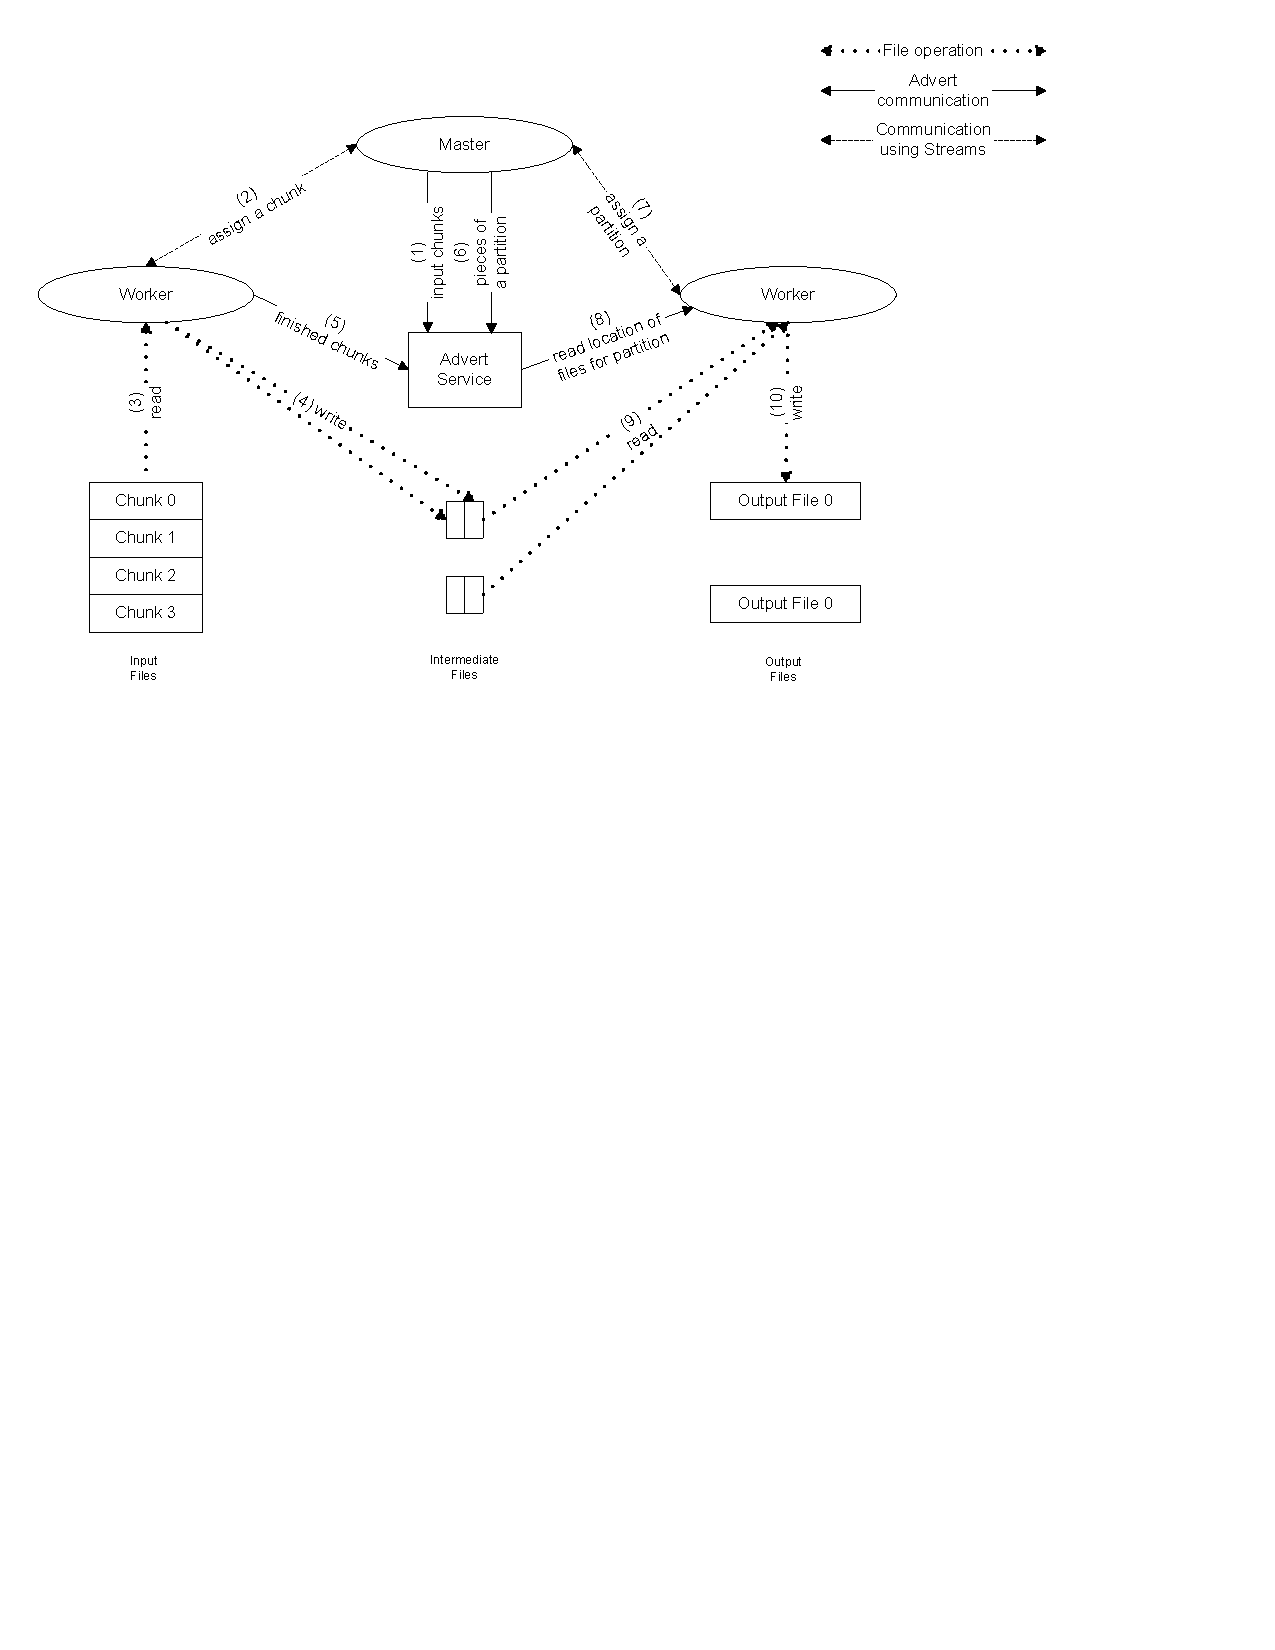
\includegraphics[width=0.5\textwidth, trim=0.5cm 17cm 3cm 0, clip]{figures/saga_mr_schema.pdf}
 \caption{
   Schema of the \sagamapreduce components and their interaction.
   \label{fig:saga_mr_schema}
   }
\end{figure}


% After \sagamapreduce we have also developed real scientific
% applications using SAGA based implementations of patterns for
% data-intensive computing: multiple sequence alignment can be
% orchestrated using the SAGA-All-pairs implementation, and genome
% searching can be implemented using SAGA-MapReduce (see
% Ref.~\cite{saga_ccgrid09}).
% \upp

\subsection{\sagamapreduce Implementation}

Our implementation of \sagamapreduce interleaves the core \mr logic
with explicit instructions on where processes are to be scheduled.
The advantage of this approach is that our implementation is no longer
bound to run on a system providing the appropriate semantics
originally required by MapReduce, and is portable to a broader range
of generic systems as well.  The drawback is that it is more
complicated to extract performance, as some system-level semantics have
to be recreated in the application space level.
The fact that the implementation is single-threaded proved to be the
primary current performance inhibitor to be addressed in the future.  However, none of these
complexities are exposed to the end-user, as they remain hidden within
the framework.

% -- for there is a need to add system
% semantic capabilities at some level, and it is inherently slower --
% as it is difficult to reproduce system-specific optimizations to
% work generically.

% Also many of the complexities are due to the early-stages of SAGA
% and incomplete implementation of features, and not a fundamental
% limitation of the design or concept of the interface or programming
% models that it supports.  Future SAGA API packages will allow to
% alleviate some of these issues.

% The overall architecture of the SAGA-MapReduce implementation is
% shown in Fig.~\ref{saga-mapreduce_controlflow}.
\smr exposes a simple interface which provides the complete
functionality needed by any MapReduce algorithm, while hiding the more
complex functionality, such as chunking of the input, sorting the
intermediate results, launching and coordinating the workers, etc. --
these are generically implemented by the framework.  The application
consists of two independent process types, a master and worker processes.
The master process is responsible for:

\begin{itemize}
 \vspace*{-0.5em}
 \setlength{\itemsep}{-.1em}


 \item launching all workers for the map and reduce steps, as
 described in a configuration file provided by the user; 
 \item coordinating the workers;
 \item chunking of the data;
 \item assigning the
 input data to the workers of the map step;
 \item handling the intermediate
 data files produced by the map step; and
 \item passing the location of the
 sorted output files to the workers of the reduce step.

% \item re-launching single worker instances in case of failures, thus
% providing fail safety.
% \miklosnote{fail safety since it's not actually present.

 \vspace*{-0.5em}
\end{itemize}

% When launching a job, the master is the executable run by the client
% itself which means the resource from which the client program is run
% determines from where the master will be available.  
Any specific MapReduce instance
is specified by a MR-JobDescription object in which the user specifies 
Mapper and Reducer classes, input and output paths and data formats.  The
used InputFormat determines the logical partitions of the input data for
the master -- that information is then sent to idle workers.  A
Raw\-Record\-Reader implementation interpretes an
InputChunk and provides a record iterator for the Mapper. It is
possible to support any kind of data source for which a record
oriented view exists, by writing a custom Raw\-Record\-Reader.
The output from the Mapper is further processed by the Partitioner
which assigns emitted key/value pairs from the Mapper to Reducers.
Finally, a Raw\-Record\-Writer writes output data to files.
% Custom
% Raw\-Record\-Writer and Partitioner classes can be also implemented to
% suit an application's needs.  \miklosnote{Andre/Shantenu: Please check
% coherence of the above paragraph.}

The master process is readily available to the user and needs no
modification to execute different map and reduce functions in the
worker processes.
% The
% worker processes get assigned work either from the map or the reduce
% step.
The \textit{functionality} for the different steps have to be provided by
the user, which means the user has to write the C++ functions
implementing the respective MapReduce kernels.

Both the master and the worker processes use the SAGA-API as an
abstract interface to the  infrastructure, making the application
portable between different architectures and systems.  The worker
processes are launched using the SAGA job package, allowing the jobs
to launch on any backend supported by SAGA (such as locally, globus/GRAM, 
EC2, SSH, Condor etc.).  The communication between the master and workers
is ensured by using the SAGA advert package, abstracting an
information database in a platform independent way, and the SAGA stream
package, abstracting streaming data access between network endpoints.
The master creates logical partitions of the data (referred to as chunking,
analogous to Google's MapReduce), so the data-set does not have to be split
and distributed manually.  The input data can be located on any file system
supported by SAGA, such as the local file system, or a distributed file system
like HDFS or KFS \cite{KFS}.


\subsection{Improving SAGA-based Map-Reduce Performance}

% \jhanote{From e-mail of 08Oct: Miklos will commit the plots, and
%   update the description of the enhanced MR to meet referee comments
%   etc. as well a brief paragraph ofhow we can in future use async
%   communication to improve the implementation of MR when using advert
%   service. All of this should be in 2-3 paragraphs or so. Also, if we
%   could have a schematic of SAGA-MapReduce that will be useful}

The performance enhancements to the \sagamapreduce implementation as
used and discussed in~\cite{saga_ccgrid09} are based on two important
changes: (i) optimizing how sorting is done after the map phase,
% \jhanote{shuffle phase has not been defined} \miklosnote{true; will
%   use other wording}
and (ii) using a serialized binary format instead
of plain text for intermediate data storage (also available as
input and output format). We expected those improvements to have
a relatively small implementation effort, and to show a significant 
impact on performance.  The first change means that,
instead of having the master merge and then sort the intermediate data
by key before entering the reduce phase, the workers buffer key/value
pairs from the map phase and store them in sorted order on disk, doing
an in-memory sort before writing. Also, since intermediate key/value
pairs from a map worker are already sorted, the reduce workers need to
only merge these pairs coming from different map workers, by
applying the user-defined reduce function to the merged intermediate
key and value list. 

The second enhancement applies to the storage of
the intermediate key/value pairs in a so-called \emph{sequence file
  format}. This file format allows storing of serialized key/value
objects which can be read and merged much faster in the reduce phase
than text data, as there is no need for costly parsing.  We used the
Google Protocol Buffers library for implementing
serialization~\cite{protobuf}. The processing of input and output
key/value pairs is further enhanced by minimizing unnecessary memory
I/O operations, using a zero-copy scheme.

% \jhanote{(A) Why do we think these are the most important performance
%   enhancements that should be attempted? Or was/is it a case of -- we
%   can, therefore we do? (B) Can the performance improvement that arise
%   from (i) and (ii) be quantified separately?  (C) What other
%   improvements can be and should be implemented?}


\subsection{\sagamapreduce Set-Up}

As with any application which concurrently spans multiple diverse
resources or infrastructures, the coordination between the different
application components becomes challenging.  The \smr implementation
uses the SAGA advert API for that task, and can thus limit the a-priori
information needed for bootstrapping the application: the compute
clients (workers) require (i) the contact URL of the used advert
service instance, and (ii) a unique worker ID to register with in that
advert service, so that the master can start to assign work items.
Both information are provided by the master via command line
parameters to the worker, at startup time.

The master application requires the following additional information:
(i) a set of resources to execute the workers on, (ii) the
location of the input data, (iii) the target location for the output
data, and (iv) the contact URL for the advert service for
coordination and communication.

For example: in a typical configuration, three worker instances may
be started; the first could be started via GRAM and PBS on
qb.teragrid.org, the second on a pre-instantiated EC2 image
(with known instance id), and the third on a dynamically deployed
EC2 instance (no instance id given).  Note that the startup times for
the individual workers may vary over several orders of magnitudes,
depending on PBS queue waiting time and VM startup time.  
That mechanism both minimizes time-to-solution, and
maximizes resilience against worker loss.
%
% The scheme \T{any} acts here as a placeholder for SAGA, so that the
% SAGA engine can choose an appropriate adaptor.  The master would
% access the file via the default local file adaptor.  The globus
% clients may use either the GridFTP or SSH adaptor for remote file
% success (but in our experimental setup would also succeed using the
% local file adaptor, as the Lustre FS is mounted on the cluster
% nodes), and the EC2 workers would use the ssh file adaptor for
% remote access.  Thus, the use of the placeholder scheme frees us
% from specifying and maintaining a concise list of remote data access
% mechanisms per worker.  Also, it facilitates additional resilience
% against service errors and changing configurations, as it leaves it
% up to the SAGA engine's adaptor selection mechanism to find a
% suitable access mechanism at runtime.  A parameter not shown in the
% above configuration example
%
A parameter controls the number of workers created per compute node;
varying that parameter permits compute and communication interleaving,
which may lead to an increase in the overall system utilization (even
in the absence of precise knowledge of the target system).

Future enhancements to \sagamapreduce might include asynchronous master-worker
communication, and off-loading coordination tasks from the advert service to
a stream-based protocol.  For example, information about the pieces of
intermediate data to be processed in the reduce phase could be directly
interchanged via streams.  The advert service could be used for maintaining
master state, in order to make the master failure-recoverable.


\section{Application Level Interoperability: Three-levels}
\label{sec:interop}

The motivation of ALI across multiple, heteregenous and distributed
resources follows from large-scale scientific applications, such as
the Earth Science Grid and LEAD. However for simplicity of treatment
and to focus on the levels of interoperability, we will use a simple,
self-contained application, that has also become the {\it canonical}
\mr application-driver -- \wc.

\subsection{Application: \Wc}
\label{ssec:app}

We use our own implementations of the well known \wc application for
our experiments.  \Wc has a well understood runtime and scaling
behaviour, and thus serves us well for focusing the tests on the used
frameworks and middlewares.

The \mr based \wc implementation is described in~\cite{saga_ccgrid09}.
For the SAGA-Sphere version of \wc we implemented two kernel
functions. The first one is responsible for hashing the
words in the data set into different "buckets". The standard C++ 
collate hashing function was used for this purpose.  The second 
kernel function reads each hash bucket, sorts the words in memory 
and outputs the final count of the words in the data set.  For example, 
a file containing the words
\T{('bread' 'bee' 'bee' 'honey')} would be hashed into buckets as
\T{('bread' 'bee' 'bee')} and \T{('honey')}.  The second kernel
function would read these intermediate bucket files, sort the words,
and produce the result \T{('bread 1', 'bee 2', 'honey
  1')}.  The Sphere system is responsible for assigning files for
processing, synchronization, and writing output results back to
Sector.

\subsection{Interoperability Types}

Using the \wc application, we will demonstrate three types of
application level interoperability. We outline them here:

% different levels/types of interoperability.

\subsubsection{Type I: Application Interoperability via adaptors}
%
% Type I:  Application
%              |
%           SAGA-MR
%              |
%           Adaptors
%      /     /   \      \
%    ... Clouds  Grids ...
%

As discussed, SAGA provides the ability to load a wide-range of
system-specifc adaptors dynamically. Thus a simple form of
interoperability, possibly specific to applications developed using
SAGA, is that an application can use any distributed system without
changes to the application, thus experiencing cloud-cloud or
grid-cloud interoperability.  We refer to this as Type I
interoperabilty.

% interoperability quite trivially thanks to the dynamic loading of
% adaptors.  A

Thanks to the relative simplicity of developing SAGA adaptors, SAGA
has been successful interfaced to three cloud systems -- Amazon's EC2,
Eucalyptus~\cite{eucalyptus} (a local installation of Eucalyptus at
LSU) and Nimbus~\cite{nimbus}; and also to a multitude of grid based
environments, including TeraGrid, LONI and NGS.  SAGA based
applications are thus inherently able to utilize this form of ALI.

\subsubsection{Type II: Application Interoperability using programming
  models} % suited for different infrastructure}
%
% Type II:      Application
%                    |
%          Instance-1 Instance-2
%            |            |
%         SAGA-Sphere SAGA-MapReduce
%            |            |
%       Sector-Sphere cluster/grids
%

Interoperabilty at a higher level than adaptors is both possible and
often desirable. An application can be considered interoperable if it
is able to switch between backend specific programming models.  We
will discuss an example where the \wc application is implemented so
that it can utilize either a Sector-Sphere framework via SAGA, or the
\smr framework for generic grid and cloud backends. \amnote{will we?}

\subsubsection{Type III: Application Interoperability using different
  programming models for concurrent execution}
%
% Type III:   Application
%                 |
%     SAGA-Sphere / SAGA-MapReduce
%                 |
%   Sector-Sphere / cluster / grids / clouds
%

At another level, an application can also be considered interoperable
when it executes multiple programming models \I{concurrently} over
diverse backends; this provides an opportunty for infrastructure
specific performance utilization.  We demonstrate that a \wc
application uses both Sector-Sphere and \smr when spanning multiple
backends \amnote{do we?}.  The challenges of having different parts of
an application execute concurrently using different programming models
is conceptually different to loading different adaptors concurrently.
Thus we describe this as a separate type of interoperability.

\subsection{Experimental Setup}

Simulations were performed on shared TeraGrid-LONI (Louisiana Optical
Network Initiative)~\cite{loni-url} resources running Globus and ssh;
on GumboGrid, a small cluster at LSU running Eucalyptus; on Amazon's
EC2; and on a bare 50 node cluster of the Hungarian Academy of Sciences;
A significant set of experiments were performed on FutureGrid
(\url{http://www.futuregrid.org}) and its IBM iDataPlex (India), which
as 256/1024 nodes/cores (for full details see:
\url{http://futuregrid.org/hardware}).

Jobs are started via the respectively available middleware, via
SAGA's job API.  Data exchange is either performed via streams, or via
SAGA's file transfer API, which can dynamically switch between the
various available protocols \jhanote{Name the protocols used
  explicitly}

For cloud environments, we support the runtime configuration of VM
instances by staging a preparation script to the VM after its
creation, and executing it with root permissions.  In particular for
apt-get \jhanote{What is apt-get?} Linux distribution, the
post-instantiation software deployment is actually fairly painless,
but naturally adds a significant amount of time to the overall VM
startup (which encourages the use of preconfigured images).

For experiments in this paper, we prepared custom VM images with
pre-installed prerequisites.  We utilize preparation scripts solely
for some fine tuning of parameters: for example, to deploy custom
saga.ini files, or to ensure the finalization of service startups
before application deployment.

Deploying \sagamapreduce framework and the \wc application on
different grids, clouds or clusters requires adapting the configuration
to the specific environment.  For example, when running \sagamapreduce
on EC2, the master process resides on one VM, while workers reside on
different VMs.  Depending on the available adaptors, Master and Worker
can either perform local I/O on a global/distributed file system, or
remote I/O on a remote, non-shared file system.

It must be noted that we utilized different \smr versions for the
described experiments: the work described in this paper spans more
than 18 months, and the \smr implementation has simply evolved over
time.  As our primary goal is to demonstrate interoperability, and not
to document maximal performance, we consider those results valid
nonetheless.


\section{Experiments}
\label{sec:exp}

\subsection{Type I ALI: Interoperability via Adaptors}

In Ref.~\cite{saga_ccgrid09}, we performed tests to demonstrate how
\sagamapreduce utilizes different infrastructures and provides control
over task-data placement; this led to insight into performance on
``vanilla'' grids.  The work presented here extends this, and
establishes that \sagamapreduce can provide cloud-cloud
interoperability and cloud-grid interoperability.  We performed the
following experiments:

\begin{enumerate}

 \item We compare the performance of \sagamapreduce when exclusively
 running on a cloud platform to that when on grids. We vary the number
 of workers (1 to 10) and the data-set sizes varying from 10MB to 1GB.

 \item For clouds, we then vary the number of workers per VM, such
 that the ratio is 1:2 and 1:4, respectively.

 \item We then distribute the same number of workers across two
 different clouds - EC2 and Eucalyptus.

 \item Finally, for a single master, we distribute workers across
 grids (QueenBee on the TeraGrid) and clouds (EC2 and Eucalyptus) with
 one job per VM.

\end{enumerate}

It is worth reiterating, that although we have captured concrete
performance figures, it is not the aim of this work to analyze the
data and provide a performance model. In fact it is difficult to
understand performance implications, as a detailed analysis of the
data and understanding the performance will involve the generation of
``system probes'', as there are differences in the specific cloud
system implementation and deployment.  In a nutshell without adjusting
for different system implementations, it is difficult to rigorously
compare performance figures for different configurations on different
machines. At best we can currently derive trends and qualitative
information.  Any further analysis is considered out of scope for this
paper.

It takes SAGA about 45s to instantiate a VM on Eucalyptus and about
200s on average on EC2.  We find that the size of the image (say 5GB
versus 10GB) influences the time to instantiate an image, but is
within image-to-image instantiation time fluctuation.  Once
instantiated, it takes from 1-10s to assign a job to an existing VM on
Eucalyptus, or EC2.  The option to tie the VM lifetime to the
\T{saga::job\_service} object lifetime is a configurable option.  It
is also a matter of simple configuration to vary how many jobs (in
this case workers) are assigned to a single VM:  the default is 1
worker per VM.  The ability to vary this number is important -- as
details of actual VMs can differ as well as useful for our
experiments.


\subsubsection*{Results and Analysis}

The total time-to-solution ($T_s$) of a \sagamapreduce job can be
decomposed as the sum of three primary components -- $t_{pre},
t_{comp}$ and $t_{coord}$.  Here $t_{pre}$ is defined as
pre-processing time, which covers the time to chunk the data into
fixed size data units, to distribute them, and also to spawn the job.
$t_{pre}$ does not include the time required to start VM instances.
$t_{comp}$ is the time to actually compute the map and reduce function
on a given worker, whilst $t_{coord}$ is the time taken to assign the
payload to a worker, update records and to possibly move workers to a
destination resource; in general, $t_{coord}$ scales as the number of
workers increases.

Table~\ref{tab:1a} shows performance measurements for a variety of
worker placement configurations.  The master places the workers on
either clouds or on the TeraGrid (TG). The configurations -- separated
by horizontal lines, are classified as either all workers on the TG or
having all workers on EC2. For the latter, unless otherwise indicated
parenthesis, every worker is assigned to a unique VM. In the final set
of rows, the number in parenthesis indicates the number of VMs used.
Note that the spawning times depends on the number of VMs, even if it
does not include the VM startup times.


Table~\ref{tab3} shows data from our interoperability tests.  The
first set of data establishes cloud-cloud interoperability. The second
set (rows 5--11) shows interoperability between grids-clouds (EC2).
The experimental conditions and measurements are similar to Table 1.

\begin{table}[h!]
  \footnotesize
  \begin{tabular}{cccccc}
    \hline
    \multicolumn{2}{c}{\#workers}  &  Data size   &  $T_s$  & $T_{sp}$ & $T_s - T_{sp}$\\
    TG &  AWS &   (MB)  & (sec) & (sec)  & (sec) \\
    \hline
  %  \textcolor{blue}{4} & - & 10  &  8.8 &  6.8 & 2.0 \\
    { {\bf 4}} & - & 10  &  8.8 &  6.8 & 2.0 \\
  %  \textcolor{blue}{6} & - & 10  &  12.4 &  10.2 & 2.2 \\
  %  10 & -  & 100 & 10.4 & 8.86 \\
  %  \textcolor{blue}{10} & - & 10  & 20.8 & 17.3 & 3.5 \\
    \hline
    - & 1 & 10 & 4.3 & 2.8 & 1.5 \\
    - & 2 & 10 & 7.8 & 5.3 & 2.5 \\
    - & 3 & 10 & 8.7 & 7.7 & 1.0 \\
    - & {\bf 4} & 10 & 13.0 & 10.3 & 2.7 \\
    - & 4 (1) & 10 & 11.3 & 8.6 & 2.7 \\
    - & 4 (2) & 10 & 11.6 & 9.5 & 2.1 \\
    \hline
    -  & 2  & 100 & 7.9  & 5.3 & 2.6 \\
    -  & {\bf 4}  & 100 & 12.4 & 9.2 & 3.2\\
    -  & 10 & 100 & 29.0 & 25.1 & 3.9 \\
    \hline
    - & {\bf 4 (1)} & 100 & 16.2 & 8.7 & 7.5 \\
    - & {\bf 4 (2)} & 100 & 12.3 & 8.5 & 3.8 \\
    - & 6 (3) & 100 & 18.7 & 13.5 & 5.2\\
    - & 8 (1) & 100 & 31.1 & 18.3 & 12.8 \\
    - & 8 (2) & 100 & 27.9 & 19.8 & 8.1\\
    - & 8 (4) & 100 & 27.4 & 19.9 & 7.5\\
    \hline \hline
  \end{tabular}
  \caption{Performance data for different configurations of worker
  placements.
  \label{tab:1a}}
\end{table}

\newpage
We find that in our experiments $t_{comp}$ is typically greater than
$t_{coord}$, but when the number of workers gets large, and/or the
computational load per worker small, $t_{coord}$ can dominate
(internet-scale communication) and increase faster than $t_{comp}$
decreases, thus overall $T_s$ can increase for the same data-set size,
even though the number of independent workers increases.  The number
of workers associated with a VM also influences the performance, as
well as the time to spawn; for example -- as shown by the three lower
boldface entries in Table 1, although 4 identical workers are used
depending upon the number of VMs used, $T_c$ (defined as $T_S -
T_{spawn} $) can be different.  In this case, when 4 workers are
spread across 4 VMs (i.e. default case), $T_c$ is lowest, even though
$T_{spawn}$ is the highest; $T_c$ is highest when all four are
clustered onto 1 VM. When exactly the same experiment is performed
using data-set of size 10MB, it is interesting to observe that $T_c$
is the same for 4 workers distributed over 1 VM as it is for 4 VMs,
whilst when the performance for the case when  4 workers are
spread-over 2 VMs out-perform both (2.1s).

Table~\ref{tab3} shows performance figures when equal number of workers are
spread across two different systems; for the first set of rows,
workers are distributed on EC2 and Eucalyptus. For the next set of
rows, workers are distributed over the TG and Eucalyptus, and in the
final set of rows, workers are distributed between the TG and EC2.
Given the ability to distribute at will, we compare performance for
the following scenarios: (i) when 4 workers are distributed equally
(i.e., 2 each) across a TG machine and on EC2 (1.5s), with the
scenarios when, (ii) all 4 workers are either exclusively on EC2
(2.7s), (iii) or all workers are on the TG machine (2.0s) (see Table
1, boldface entries on the first and fifth line). It is {\it
  interesting} that in this case $T_c$ is lower in the distributed
case than when all workers are executed locally on either EC2 or TG;
we urge that not too much be read into this, as it is just a
coincidence that a {\it sweet spot} was found where on EC2, 4 workers
had a large spawning overhead compared to spawning 2 workers, and an
increase was in place for 2 workers on the TG. Also it is worth
reiterating that for the same configuration there are
experiment-to-experiment fluctuations (typically less than 1s).  The
ability to enhance performance by distributed (heterogeneous)
work-loads across different systems remains a distinct possibility,
however, we believe more systematic studies are required.

\begin{table}[h!]
  \footnotesize
  \begin{tabular}{ccccccc}
    \hline
    \multicolumn{3}{c}{\# workers}  &  Size   &  $T_s$  & $T_{sp}$ & $T_s - T_{sp}$\\
    TG &  AWS & Eucal. &  (MB)  & (sec) & (sec) & (sec) \\
    \hline
    - & 1 & 1 & 10   & 5.3 & 3.8 & 1.5\\
    - & 2 & 2 & 10   & 10.7 & 8.8 & 1.9 \\
    - & 1 & 1 & 100  & 6.7 & 3.8 & 2.9\\
    - & 2 & 2 & 100  & 10.3 & 7.3 & 3.0\\
    \hline
    1 & - & 1 & 10   & 4.7 & 3.3 & 1.4\\
    1 & - & 1 & 100  & 6.4 & 3.4 & 3.0\\
    \hline
    {\bf 2} &   {\bf 2} & - & 10 & 7.4 & 5.9 & 1.5 \\
    3 & 3 & - & 10 & 11.6 & 10.3 & 1.6 \\
    4 & 4 & - & 10 & 13.7 & 11.6 & 2.1 \\
    5 & 5 & - & 10 & 33.2 & 29.4 & 3.8 \\
  %\textcolor{blue}{5} & \textcolor{blue}{5} & - & 10 & 33.2 & 29.4 & 3.8 \\
    10 & 10 & - & 10 & 32.2 & 28.8 & 2.4 \\
    \hline
     \hline
  %   1 & 1 & - & 100 & 5.4 & 3.1 & 2.3\\
  %   3 & 3 & - & 100 & 11.1 & 8.7 & 2.4 \\
  \end{tabular}
  \caption{Performance data for different configurations of worker
  placements on TG, Eucalyptus-Cloud and EC2.
  \label{tab3}}
\end{table}

The original \sagamapreduce version (as used for the experiments
presented above) physically chunked the input data files.  Our evolved
version, however, creates logical chunks (i.e., no file
writing takes place).  It is thus fair to compare their
time-to-solution performance by subtracting the chunking time from the
early-version's job completion time.  Fig.~\ref{fig:sagamr_comparison}
shows the thus corrected performance data for the early-version and
enhanced version of \sagamapreduce.  8 workers were spawned via the
SAGA SSH adaptor on 8 physical machines,  data were exchanged through
a shared NFS file system.  The figure shows that the \sagamapreduce
enhancements make a difference for larger data sets.  This can be
attributed to the fact that the more efficient shuffle phase
implementation, which reduces disk I/O and CPU usage in the reduce
phase by doing only a merge, outperforms the old implementation, which
performed a merge-sort of all the intermediate output files.

\begin{figure}[htb!]
 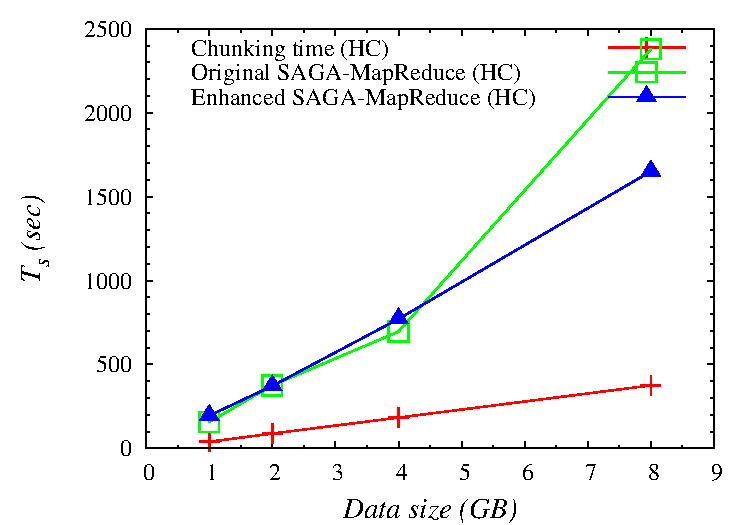
\includegraphics[width=0.5\textwidth]{figures/sagamr_comparison.pdf}
 \caption{Comparison of enhanced SAGA-MR performance versus
   early-version of SAGA-MR on HC using 8 workers running on 8
   physical machines. Jobs were launched via SSH and used NFS for file
   operations. Chunking data shown here is for the original
   \sagamapreduce.} \label{fig:sagamr_comparison}
\end{figure}


\subsection{Type II ALI: Application Performance Using SAGA-based
Sphere and MapReduce}

The various experiments described in this section have been performed
in two configurations -- determined by the distribution (or lack
thereof) of the computational resources and data-access method. In the
first configuration (``local''), all application processes used a
single compute node, with local data access.  In the second
configuration (``dist.''), the application processes were distributed
over multiple physical nodes, and utilized remote data access
techniques, such as distributed file-systems, or distributed
file-transfer. % \jhanote{Please check that this is correct.}
% \miklosnote{It's correct. However, I'm not sure if mentioning both
% file-systems and file-transfer is needed.}

\subsubsection{Experiment I -- Varying chunk sizes}

For the SAGA Sector-Sphere based \wc, Sector maintains and tracks data at
the file level. To experiment with different chunk sizes, the data
files (totalling 4GB) were split manually into smaller chunks before
the \wc application was launched. In this set of experiments, we vary
the chunk size from 16 MB to 256 MB, while keeping the number of SPEs
constant at 8, and the total data size constant at 4 GB. Each SPE is
running on a separate physical node in the cluster. These results are
presented in Fig.~\ref{fig:sphere_mr_chunksize}.  Note that both data
and computation were distributed for these experiments.

As evident from Fig.~\ref{fig:sphere_mr_chunksize}, a correlation
exists between the chunk sizes and performance of Sphere.  As the
chunk sizes increase, the time-to-solution also increases. In
particular, we observe that performance declines for chunk sizes
larger than 64 MB. On the Hungarian cluster, the time-to-solution
increased by 21 \% going from 64 MB chunk size to 128 MB chunk
size, and by 56 \% going from 128 MB chunk size to the 256 MB
chunk size. On the India system of the FutureGrid cluster, the time-to-solution increased
by 22 \% going from 64MB to 128MB and 25 \% going from 128MB
to 256MB.

% \jhanote{It is difficult to discern from the graph. Please also
%   provide a quantitative estimate of what the performance decrease is
%   after 64MB, i.e. what percent increase is there in going from
%   64-128, and 128-256} 

% \jhanote{Saurabh, please confirm that these experiments on
%   Sector/Sphere were repeated? If so, please tell me what the typical
%   variation was}
% \ssnote{Shantenu, you can look at the variations on the online spreadsheets}

\begin{figure}[htb!]
 \dnnn\dnnn
 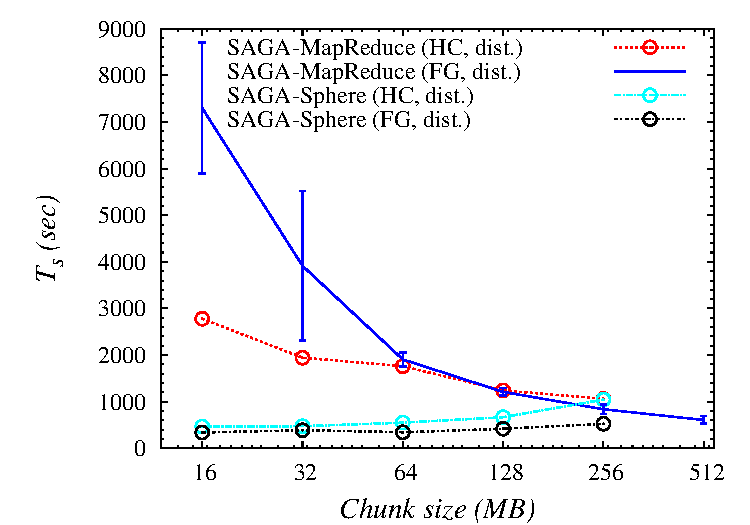
\includegraphics[width=0.5\textwidth]{figures/sphere_mr_varying_chunksize.pdf}
 \caption{
   Performance of \sagamapreduce and
   SAGA-Sphere when varying chunk size while keeping the amount
   of processed data constant at 4GBs. Data and computation were
   distributed for these experiments.
   \label{fig:sphere_mr_chunksize}
 }
\end{figure}

We performed the same set of experiments with SAGA-MapReduce based \wc
and observe a completely different performance trend as the chunk size
varied.  We use an HDFS file system running data nodes on each of the
8 workers and set the number of reduce tasks to 8.  In case of
SAGA-MapReduce, performance increases, i.e., time-to-solution
decreases, with larger chunk sizes, reaching Sphere's performance at
the 256 MB data point.

This can be attributed to the fact that for SAGA-MapReduce,
$t_{coord}$ is dominated by the number of chunks (map tasks).
%assigned to a given worker.  
The larger the chunk size, the smaller the number
of map tasks; and provided the data work-load assigned to each worker
is not too high, $t_{coord}$ decreases with decreasing number of map
tasks (increasing chunk size).

These experiments have been run on both the Hungarian cluster (HC) and
on the India system of FutureGrid (FG), which have rather different hardware
charasteristics.  The graph shows the discussed trends are independent
of the backend, and depend on the programming model used and its
implementation. The experiment's standard deviations are usually below
10\% of the measured data values, and have been plotted where they
exceed the plot point size.  For SAGA-MapReduce, the data points for
small chunk sizes varied significantly, as shown in the graphs.
The latter can be attributed to the fact that a high number of map-tasks
cause contention due to the advert service, i.e. they require higher
coordination overhead.

% \jhanote{Is this because the number of map-tasks is high and thus
%   there is contention due to the advert service? If not, we need to
%   explain why?}
% \miklosnote{Does the added sentence clarify this?}
% as dominate the total time-to-solution for large number of worker
% tasks (or equivalently smaller chunk sizes).

\subsubsection{Experiment II -- Varying Workers}

Having understood the influence of the chunk size on performance, the
next set of experiments aim to understand how varying the number of
workers effects the time-to-solution. These experiments are carried
out on both the HC and India.
Fig.~\ref{fig:sphere_varying_workers} shows the results for
SAGA-Sphere, Fig.~\ref{fig:sagamr_varying_workers} for
SAGA-MapReduce.  The chunk size was set constant at 64 MB, the data
size again 4GB.

\begin{figure}[htb!]
 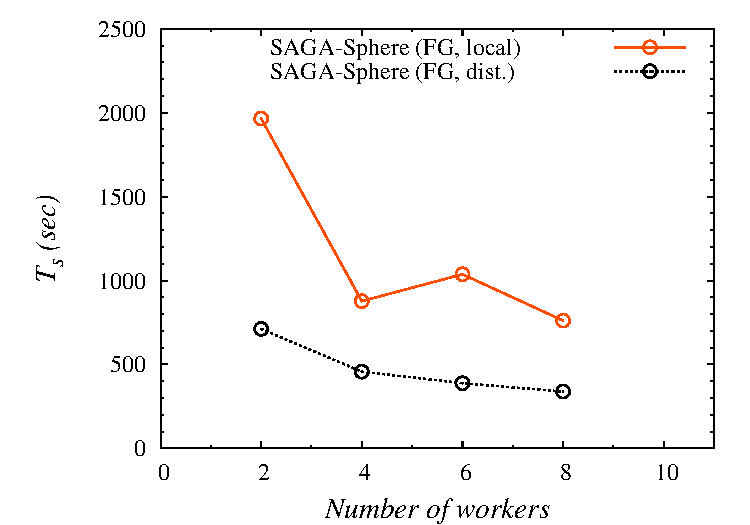
\includegraphics[width=0.5\textwidth]{figures/sphere_varying_workers.pdf}
 \caption{
   Comparison of SAGA-Sphere performance when varying the number of workers
   between 2 and 10 in two configurations: (1) local data and computation
   and (2) distributed data and computation.
   \label{fig:sphere_varying_workers}
   }
\end{figure}

\jhanote{Saurabh: Is this for FutureGrid? Please clarify} 
\ssnote{Clarified in the paragraph below}

For the local configuration, we launch Sector and Sphere on a single physical
node on the Hungarian cluster. For the distributed configuration, we 
launch Sector and Sphere on one physical node per SPE. The distributed experiments
are performed both on the Hungarian cluster and the India system of the FutureGrid cluster as well. 

For the data-set sizes considered, we observe good performance over 4 to 6 
distributed workers, after which the coordination costs due to the number of SPEs starts to get high, with
a concomitant increase in time-to-solution. This is a nice but simple
demonstration of the advantage of distribution (logically distributed
in this case, if not physically distributed). Sector can maintain file
replicas to achieve optimal data distribution between SPEs and
minimize synchronization overhead. For the purpose of our experiments,
we limited Sector to not create any replicas.

The performance on the HC for a local configuration, shows obvious
performance problems.  The hardware was, both in terms of memory and
CPU, not able to cope with the workload in that configuration.
\jhanote{Please see accompanying e-mail about using HC data in
  distributed mode?  This paragraph should go if we remove the HC data
  from Fig 5 and Fig 6.}

\begin{figure}[htb!]
 \dnnn\dnnn
 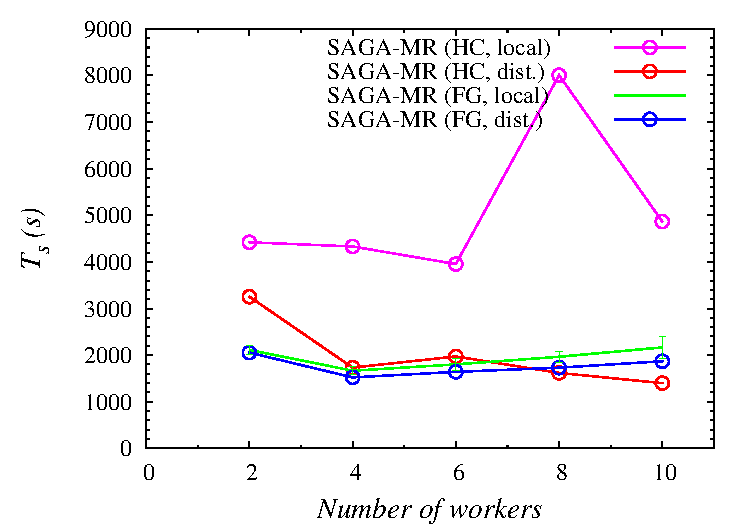
\includegraphics[width=0.5\textwidth]{figures/sagamr_varying_workers.pdf}
 \caption{ Comparison of \sagamapreduce when varying the number of
   workers between 2 and 10 in two configurations: (1) local data and
   computation and (2) distributed data and computation.
   \label{fig:sagamr_varying_workers}
   }
\end{figure}


% \jhanote{I can't determine where we establish that for varying chunk
%   size we say that the number of workers in the map phase is not the
%   same as the reduce phase. We only say that the number of reduce
%   workers is set to 8 and imply that it is kept fixed.}
 
We performed similar measurements via \sagamapreduce.  We set the
number of reduce tasks to be equal to the number of workers spawned.
For the local configuration we launch workers on the machine running
the master as separate processes and use the local file system for
file operations.  For the distributed configuration we use HDFS as the
distributed file system and launch jobs using the SAGA SSH job
adaptor. As can be seen in Fig.~\ref{fig:sagamr_varying_workers}
\sagamapreduce does not scale as expected in the distribute
configuration.  This is most likely due to the increased coordination
costs that arise with an increasing number of workers.
% \miklosnote{Explain why} \jhanote{Miklos -- is this satisfactory?}
% \miklosnote{Yes!}

Since each map task writes as many files as the number of reduce tasks
at the same time, and each reduce task needs to read from as many
files as the number of input chunks, the number of concurrent disk I/O
increases very quickly; this can cause a bottleneck when performing
computations on one physical node (I/O system).  According to
Fig.~\ref{fig:sagamr_varying_workers} the optimal number of workers
(for 4GB and a chunk size of 64MB) is 4 for the local configuration.
 
On FutureGrid, the local configuration performance shows similar
trends to the distributed configuration; there is essentially a fixed
(consistent) difference in the time-to-solution between the local and
distributed configurations. To a first approximation, this can be
explained by the fact that any gains in I/O cost by distributing data
are compensated for by the overhead of setting up the distributed
workers. This is consistent with the fact that as smaller worker
counts (and thus lower coordination and set-up overhead), the
distributed and local configurations have comparable performance.  It
is fair to assume that as data-set sizes become larger, the
distributed case will gradually perform better. %  \miklosnote{This
%   should be explained with mentioning communication cost and pointing
%   at good machine hardware which makes gains by distributing workers
%   diminishing.}\jhanote{Miklos: Please check that my explaination is
%   OK?} \miklosnote{It is OK.}

Similar to results for SAGA-Sphere, the \sagamapreduce data for the
local configuration on the HC shows the same node saturation
\jhanote{What is node saturation?} with increasing worker numbers. The
standard deviations for these runs have again been below 10\% in most
cases, and have been plotted where they exceed the plot point
size. \jhanote{As the number of workers increase, the data for
  \sagamapreduce on HC (red) varies more than 10\%.. (at 10 workers it
  is approx 1400; at 6 workers it is approximately 2000) hence the
  explanation that \sagamapreduce is the same as SAGA-Sphere is not
  rigorously true} \jhanote{Do you mean standard errors or do you mean
  standard deviation. This is important.}

\paragraph{Discussion:}
As evident from the data plots in Fig.~\ref{fig:sphere_mr_chunksize},
certain behavioral trends for SAGA-Sphere and \sagamapreduce emerge.
In Experiment 1, where we keep the number of workers constant and vary
the chunk sizes, the trends between \sagamapreduce and Sphere are
inversed: the performance of SAGA-Sphere deteriorates with increasing
chunk sizes, while the performance of \sagamapreduce improves. This
behavior suggests that \sagamapreduce's synchronization overhead to
manage smaller chunk sizes compared to the speed up achieved through
parallelism is much higher.  In the case of the \wc application,
\sagamapreduce appears to be more suitable for coarse grained
computations. SAGA-Sphere, on the other hand, yields better
performance from smaller chunks sizes (a larger amount of files)
making it suitable for finer grained computations with better data
distribution.

We instrumented the Sphere code to analyze it's behavior in more detail.
The processing of larger files (i.e. reading the file from disk to memory,
computing the hash for the words contained in the file, as
well as writing the file into the Sphere output buffer) did not
contribute significantly to the time taken for solution. We did
observe that once the Sphere framework took over the responsibility
of processing the output buffer, it took more time to process larger
buffers than smaller ones. Identifying exactly what module is
responsible for this bottleneck is out of the scope of this paper.

In Experiment 2, where we keep the chunk size constant at 64 MB,
SAGA-Sphere exhibits a trend where adding more SPEs for the distributed configuration has a positive
impact on performance. However, at the 8 SPEs and 10 SPEs data points,
we see a decline in performance, possibly due to high synchronization
costs between the workers.  What is interesting to notice are the two
data points at 128 MB chunk size and at 16 MB chunk size for
SAGA-Sphere in Fig.~\ref{fig:sphere_mr_chunksize} for the distributed HC and FG environments. Reducing the chunk
size results in a greater number of files, and thus provides
the opportunity for better data distribution; we notice an almost 30\%
improvement in performance for HC and 19\% for FutureGrid. This further confirms our supposition that
good data distribution had a major impact on Sphere's performance for
the \wc application. \jhanote{Once again the scale in Figure 4 makes
  this difficult to discern. Also we need to state whether this true
  for local, distributed or both. I think both -- but needs to be
  said}
\\ssnote{Addressed Shantenu's comment. Missed this one previously}

% We instrumented the Sphere code to analyze this behavior further.
% The processing of larger files (i.e. reading the file from disk to memory,
% computing the hash for the words contained in the file, as
% well as writing the file into the Sphere output buffer) did not
% contribute significantly to the time taken for solution. We did
% observe that once the Sphere framework took over the responsibility
% of processing the output buffer, it took more time to process larger
% buffers than smaller ones. Identifying exactly what module is
% responsible for this bottleneck is out of the scope of this paper.

We do not claim that fine grained computation granularity is a concrete
determinant of SAGA-Sphere's performance in a general case, but a
noticeable aspect that emerges through its comparison with
\sagamapreduce.


\subsection{Type III ALI: Concurrent Interoperability}

We discuss a third type of interoperability in this section, where
SAGA-MapReduce and SAGA-Sphere are used in conjunction to solve the
\wc problem. We first use the 'netperf' utility to measure the
throughput from the client host to the \sagamapreduce master node and
SAGA-Sphere master node.  In our case, the throughput measured to the
two nodes was approximately equal (935 MB/s to SAGA-Sphere and 925
MB/s to SAGA-MapReduce).  Based on these metrics, we split the 4.0 GB
data set into two equal 2.0 GB parts. This is to ensure that the data
transfer time to both masters is approximately the same. We configured
both systems to utilize 4 workers each and 64 MB chunk sizes. The data
transfer time to the Sector cloud took a total of 97.8 seconds and
10.4 seconds to the SAGA-MapReduce master node. The longer transfer
time to Sector can be credited to the overhead incurred from
registering the files in Sector. The Sector upload utility was used 
to transfer the data. 
\amnote{so, the BW measurement was for nothing after all? ;-) Also:
  what does sequentially mean here?}  \miklosnote{Should describe here
  the configurations used for Sphere and MapReduce too.}

We found that SAGA-Sphere took a total of 441.3 seconds to process the
2.0 GB data, while \sagamapreduce took a total of 769
seconds. Aggregating the output results from the two systems took a
negligible amount of time (only 0.9 seconds). The data was already
sorted and hence could be merged in almost constant
time. % O(n) complexity.
The above simple experiment of combining two varied programming models
for solving a common problem paves the way to further investigation
into smarter data and compute placement techniques.  The total time
taken to execute the \wc application in this case was approximately
877.9 seconds. It is interesting to note that this performance measure
lies between 1329.96 seconds for 8 SPEs and 716 seconds for 8
SAGA-MapReduce workers at a 64 MB chunk size.\amnote{recheck data points!}

\section{Discussion \& Conclusions}
\label{sec:discuss}

SAGA gives us the opportunity to experiment with different programming
models on different infrastructure and with varying configuration.
For example, in case of \sagamapreduce we observed that the latency of
the advert service used during computation has a significant impact on
time-to-solution. The results reported therein have been obtained by
employing an advert service solely used for our experiments.  We found
that using a publicly available one having several concurrrent users
can even double time-to-solution in configurations having high
coordination overhead, i.e., in case of a small chunk size or large
number of workers.

The aim of this paper has been to show several types (and levels) of
interoperability; although driven by proof-of-capability experiments
and results therein, there are deeper questions that motivate this
work and define the research methodology.  As alluded to in the
opening section, the volume and the degree-of-distribution of data is
increasing rapidly; this imposes a need for applications to work
across a range of distributed infrastructures using several
programming models; this is consistent with the fact that it is not
possible to localize exa-bytes of data.  Thus, on the one hand there
is a need to decouple PM from infrastructures, and provide a range of
PM at the application developer's disposal. On the other hand, in
order to build empirical models, or validate existing predictions of
performance, it is important to establish \& experiment with
programming models and data-oriented algorithms (e.g., streaming) on a
range of systems. % This is an important step towards general-purpose
% programming models, the first-step of which is interoperability of the
% types discussed.
A critical and necessary step to achieve both is to provide
application-level interoperability as discussed.

In this paper, we posit three levels of interoperability; tests at all
three levels, were performed using SAGA-\mr, which from an execution
perspective is a relatively straight-forward application.  At the
lowest level, \sagamapreduce demonstrates how to decouple the
development of applications from the deployment details of the
run-time environment (Type I ALI).  It is critical to reiterate that
using this approach, applications remain insulated from any underlying
changes in the infrastructure -- not just grids and different
middleware layers, but also different systems with very different
semantics and characteristics, whilst being exposed to the important
distributed functionality.

With implementations of the two application frameworks -- SAGA based
Sector-Sphere and the \smr implementation, we also demonstrated Type
II ALI: applications can seemlessly switch between backends by
switching frameworks encapsulating different programming models.
Finally, by concurrently using Sector-Sphere \mr and \smr, we
demonstrated Type III ALI, allowing the application to span a wide
variety of backends concurrently, and efficiently.

Our approach does not confine us to \mr and applications based upon
\mr; SAGA is also capable of supporting additional programming models,
like Dryad.  We are also developing applications with non-trivial
data-access, transfer and scheduling characteristics \& requirements,
and deploying them on different underlying infrastructure guided by
heuristics to seek optimised performance.
% We will generalize our approach to most efficiently execute it by
% taking into consideration the data-locality, as well as the access
% patterns of the execution steps required to complete the work flow.
This analysis is done through developing performance models of
transferring data between frameworks, as well as the distribution of
the computing resources in the environment. Based on this analysis,
the data is placed efficiently, and a subset of nodes and frameworks
maybe chosen to perform the necessary computations. The shuffled data
is also cached for future computations.  We have embarked on the
creation of components that facilitate intelligence and flexibility in
data placement relative to the computational resource
~\cite{saga_dic_royalsoc09}. These components are connected in
frameworks using SAGA, thus further the agenda of general-purpose
programming models with efficient run-time support that can utilize
multiple heterogeneous resources.

% -- that is either data can be transferred intelligently to match
% computational workloads or computational workloads can be placed to
% match (prevent) data requirements

% In all of this, important to distinguish the infrastructure
% independence of \sagamapreduce with the reliance of Google's
% MapReduce~\cite{mapreduce-paper} on a number of capabilities of the
% underlying system -- mostly related to file operations, but including
% system features related to process/data allocation.

% {\it Programming Models for Clouds: } Ref~\cite{jha_ccpe09} introduced
% the notion of {\it affinity} for clouds to capture the idea of
% relative data-compute placement and locality; it is imperative that
% any programming model/system be cognizant of the notion of
% affinity. We have implemented the first steps in a PM which provides
% easy control over relative data-compute placement; a possible next
% step would be to extend SAGA to directly support affinity (data-data,
% data-compute).

% More generically, it is worth mentioning that these approaches can be
% extend to support certain kinds of {\it affinities}.



% A feature worth noting in MapReduce is that the ultimate dataset is
% not on one machine, it is partitioned on multiple machines
% distributed.

% Google use their distributed file system (Google File System) to keep
% track of where each file is located.  Additionally, they coordinate
% this effort with BigTable.

% {\it Simplicity versus Completeness:} There exist both technical
% reasons and social engineering problems responsible for low uptake of
% grids. One universally accepted reason is the complexity of grid
% systems -- the interface, software stack and underlying complexity of
% deploying distributed application. But this is also a consequence of
% the fact that grid interfaces tend to be ``complete'' or very close
% thereof.  % For example, while certainly not true of all cases, consider
% % the following numbers, which we believe represent the above points
% % well: globus 4.2 provides, in its Java version,
% % approximately 2,000 distinct method calls.  The complete SAGA Core
% % API~\cite{saga-core} provides roughly 200 distinct method calls.
% % The
% % SOAP rendering of the Amazon EC2 cloud interface provides,
% % approximately 30 method calls (and similar for other Amazon cloud
% % interfaces, such as Eucalyptus~\cite{eucalyptus}).
% The number of
% calls provided by these interfaces is no guarantee of simplicity of
% use, but is a strong indicator of the extent of system semantics
% exposed.  But to a first approximation, (simplicity of) interface
% determines the programming models that can be supported. Thus there is
% the classical trade-off between simplicity and completeness.

%\section{Conclusion and Some Future Directions}

% EC2 and Eucalyptus although distinct systems
% have similar interfaces; we will work towards developing SAGA based
% applications that can use very different infrastructures, e.g.,
% Google's AppEngine, such that \sagamapreduce uses Google's cloud
% infrastructure.

% Finally, it is worth mentioning that computing in the clouds for
% this project cost us upwards of \$300 to perform these experiments
% on EC2.

%   somewhat similar; a very different beast is Google's AppEngine.  We
%   will in the near future be working towards providing \sagamapreduce
%   via Google's AppEngine

% {Mention that Amazon and Eucalyptus although distinct are
%   somewhat similar; a very different beast is Google's AppEngine.  We
%   will in the near future be working towards providing \sagamapreduce
%   via Google's AppEngine}


% Patterns capture a dominant and recurring computational mode; by
% providing explicit support for such patterns, end-users and domain
% scientists can reformulate their scientific problems/applications so
% as to use these patterns.  This provides further motivation for
% abstractions at multiple-levels.


%\section{Acknowledgments}
\subsection*{Acknowledgments}

\small{SJ acknowledges UK EPSRC grant number GR/D0766171/1 for
  supporting SAGA and the e-Science Institute, Edinburgh for the
  research theme, ``Distributed Programming Abstractions''.  SJ also
  acknowledges financial support from NSF-Cybertools and NIH-INBRE
  Grants, while ME acknowledges support from the grant OTKA NK 72845.
  We also acknowledge internal resources of the Center for Computation
  \& Technology (CCT) at LSU and computer resources provided by
  LONI/TeraGrid for QueenBee.  We thank Chris Miceli, Michael Miceli,
  Katerina Stamou \& Hartmut Kaiser for their collaborative efforts on
  early parts of this work. We thank Mario Antonioletti and Neil Chue
  Hong for supporting this work through GSoC-2009 (OMII-UK Mentor
  Organization). This document was developed with support from the
  National Science Foundation (NSF) under Grant No. 0910812 to Indiana
  University for "FutureGrid: An Experimental, High-Performance Grid
  Test-bed." Any opinions, findings, and conclusions or
  recommendations expressed in this material are those of the
  author(s) and do not necessarily reflect the views of the NSF.}

\bibliographystyle{plain}
\bibliography{saga_data_intensive}

\end{document}

% This work would not have been possible without the efforts and
% support of other members of the SAGA team.  In particular,
% \sagamapreduce was originally written by Chris and Michael Miceli,
% as part of a Google Summer of Code Project, with assistance from
% Hartmut Kaiser. We also thank Hartmut for great support during the
% testing and deployment phases of this project. We are greatful to
% Dmitrii Zagorodnov (UCSB) and Archit Kulshrestha (CyD group, CCT)
% for the support in deployment with Eucalyptus.  KS would like to
% acknowledge the LSU Networking Infrastructure \& Research IT
% Enablement team for their help and support.

% We % did not include results for more than 10 workers in order to 
% preserve the linear scale. 
%
% \miklosnote{Shall we note why we don't include results for 10
%   workers in the local configuration (takes toooooo much
%   time)?} \jhanote{done} \amnote{does not add up IMHO, and rather 
%   confuses}
